\documentclass[../../main]{subfiles}
\begin{document}
\subsection{General model}
\label{ch:General_model}

In this project a pan-tilt system has been given to control. This can be seen on figure \ref{fig:ImageOfPanTiltSystem}.

\begin{figure}[h]
  \centering
  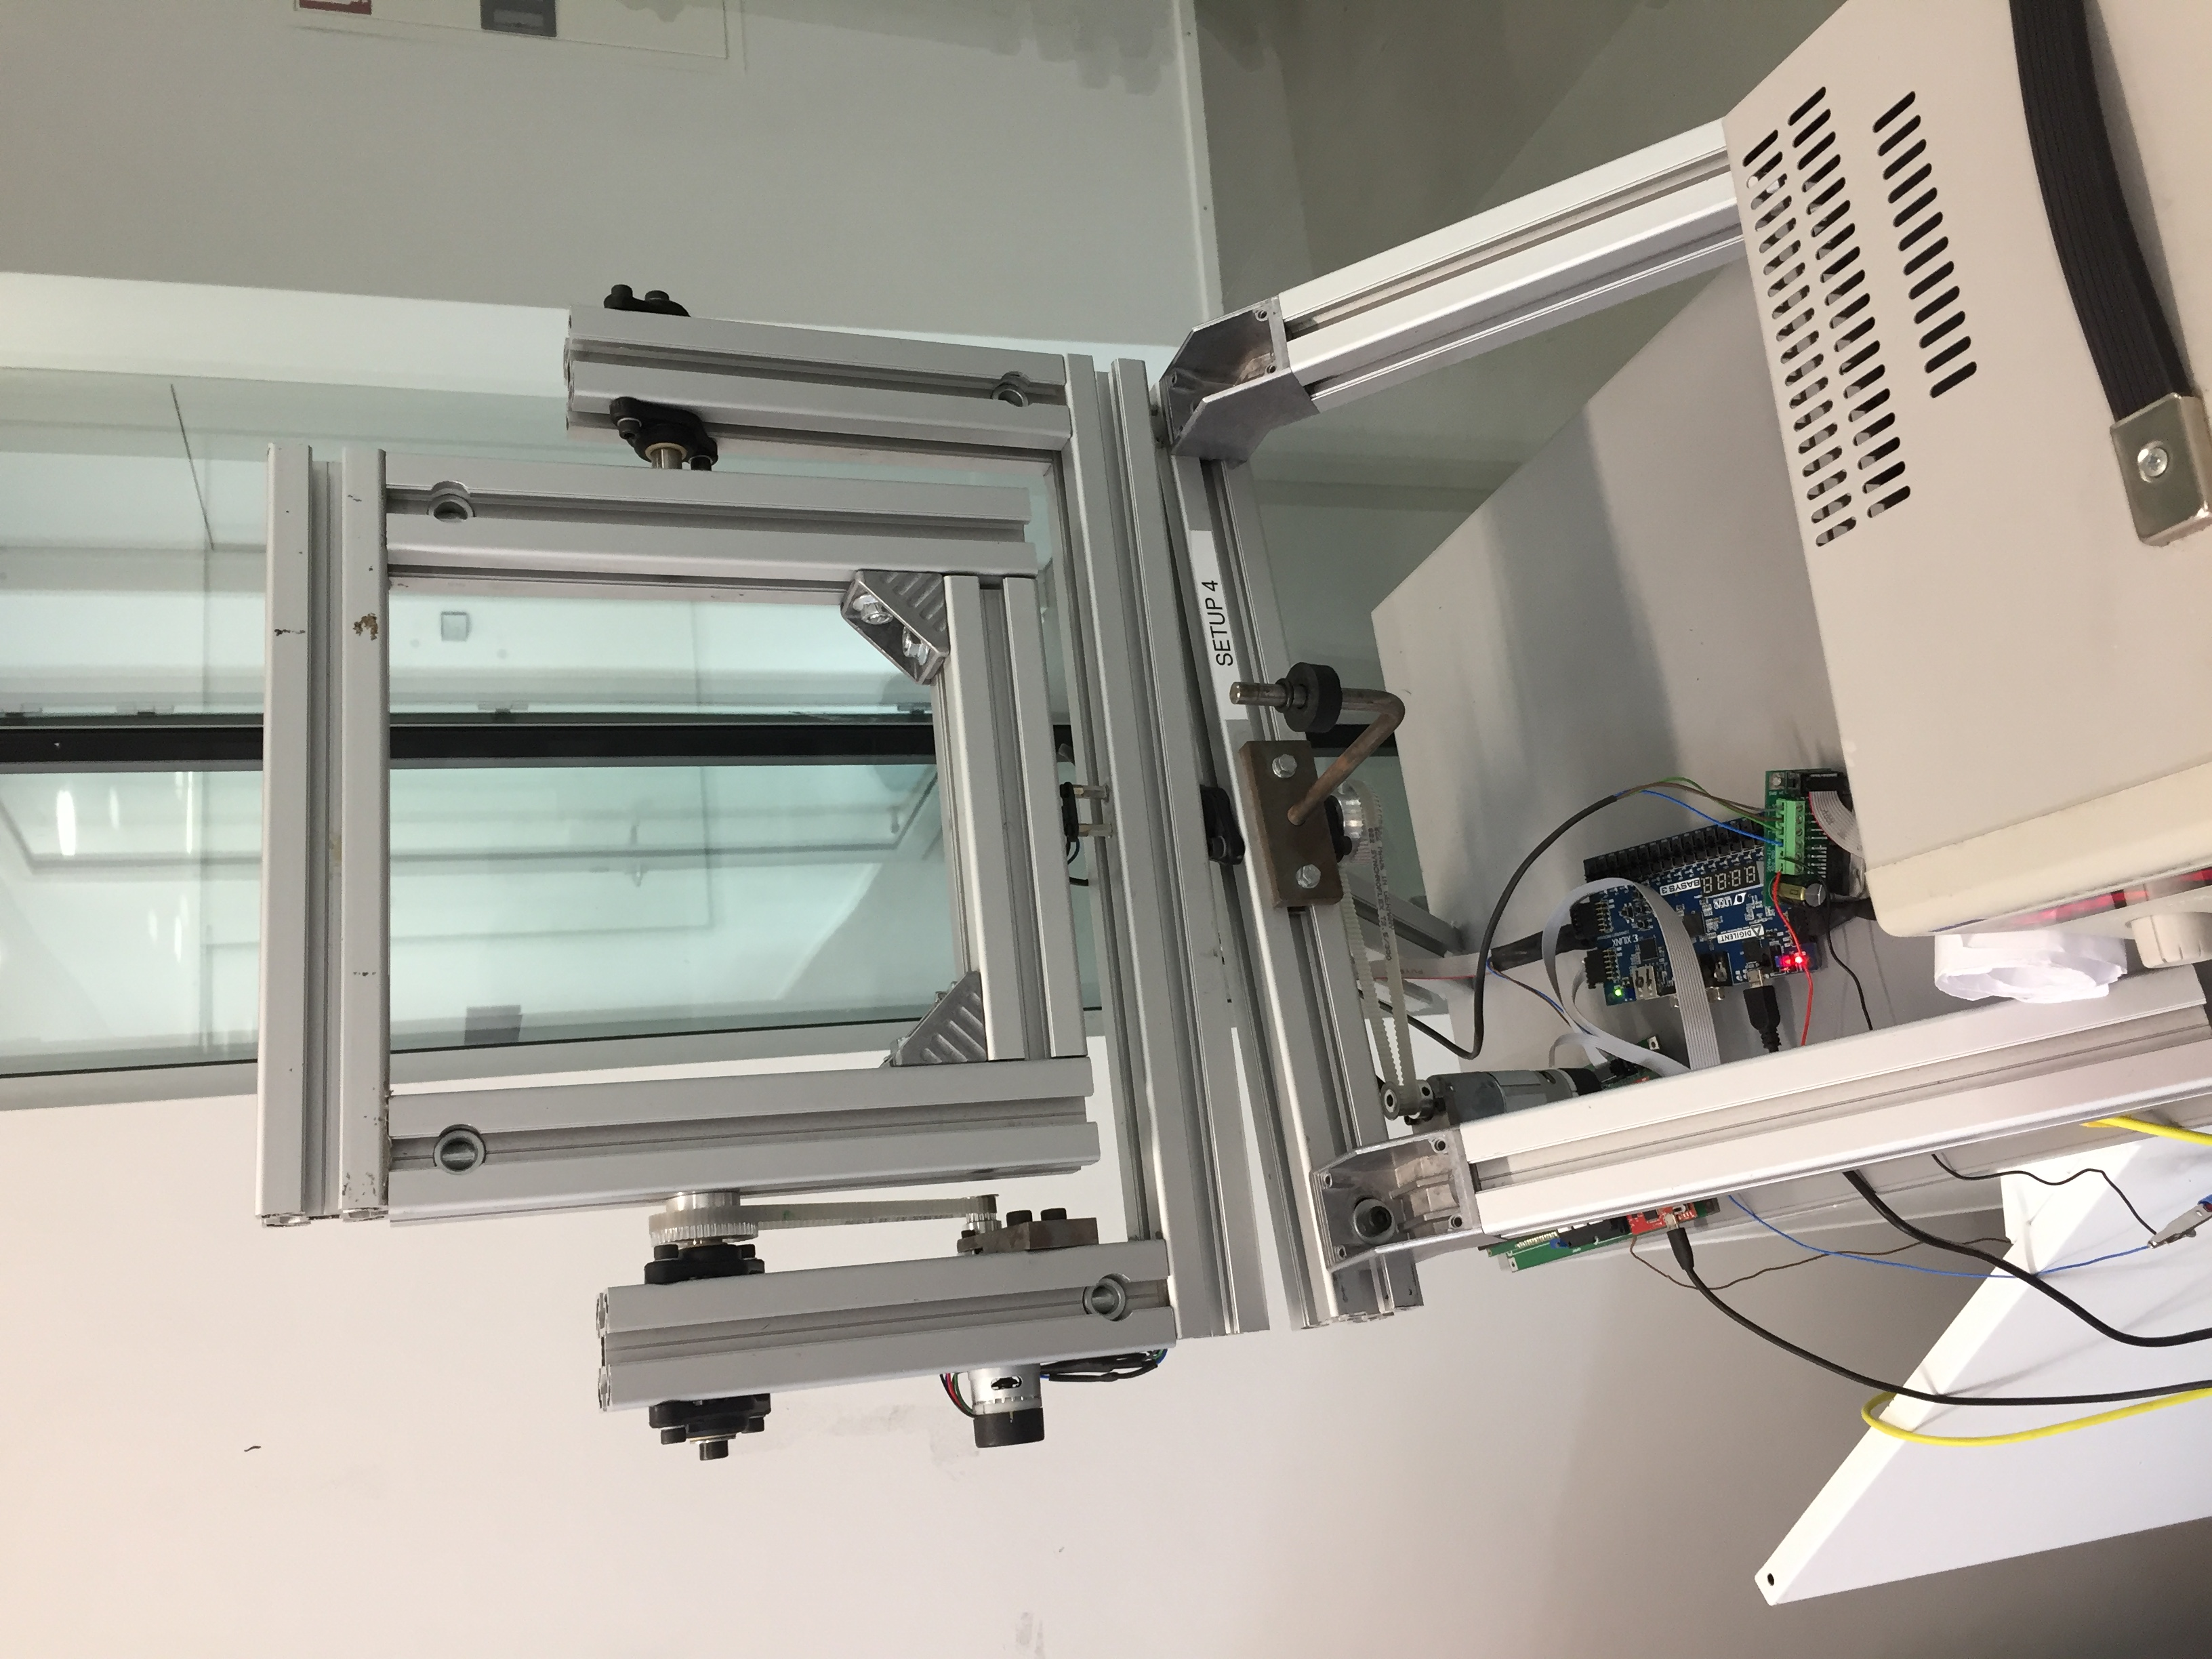
\includegraphics[width = 0.5\textwidth, angle = 270]{\main/ImageOfPanTiltSystem.JPG}
  \caption{Image of the pan-tilt system given.}
  \label{fig:ImageOfPanTiltSystem}
\end{figure}

The system works such that the upper frame is driven by a motor causing it to rotate about a horizontal axis, while the buttom frame is driven by a similar motor but has a veritkal axis. This can be seen illustrated on figure \ref{fig:pan-tilt_frames}.

  \begin{figure}[h]
    \centering
  \def\svgwidth{0.4\columnwidth}
  \subfloat[Top frame of the pan-tilt system.]{\includesvg[\main/afsnit/system_modeling/]{TopFrame_general}}\qquad
  \def\svgwidth{0.2\columnwidth}
  \subfloat[Bottom frame of the pan-tilt system.]{\includesvg[\main/afsnit/system_modeling/]{ButtomFrame_general}}
  \caption{Pan-tilt frames.}
  \label{fig:pan-tilt_frames}
  \end{figure}

In this chapter an approximated model of the physical system will be found.\\

By analysis of the forces acting on the motors when voltage is added, the following differential equations are found.\\

\begin{equation}
  \label{equ:model_mech_equ}
  J\cdot \ddot \theta + b\cdot \dot \theta = K_{torque}\cdot i
\end{equation}

\begin{equation}
  \label{equ:model_ele_equ}
  L\cdot \frac{di}{dt} + R\cdot i = V - K_{elec}\cdot \dot \theta
\end{equation}

In (\ref{equ:model_mech_equ}) $J$ is the moment of inertia about the axis of rotation, $b$ is the motors viscous friction constant, $K_{torque}$ is the motor toque constant, $\dot \theta$ is the first time derivative of the position, and $\ddot \theta$ is the second time derivative. The first time derivative is this the velocity and the second is the acceleration.\\
In (\ref{equ:model_ele_equ}) $L$ is the electrical inductance of the coil in the motor, $\frac{di}{dt}$ is the first time derivative of the current, $R$ is the ohmic resistance of the motor, $V$ is the voltage applied, $K_{elec}$ is the electromotive force constant and as mentioned above $\dot \theta$ is the velocity.\\

By further inspection a non-linear contribution on the top frame's moment of inertia is caused by the added aluminium corners as seen on figure (\ref{fig:real_image_of_pan-tilt_system}).\\
Adding the extra gravitational pull on these corners, the mechanical equation describing the motor driving the top frame can be rewritten as seen in eq. (\ref{eq:new_mech_equation_with_corners}).

\begin{equation}
  \label{eq:new_mech_equation_with_corners}
  J_t\cdot \ddot \theta_t + b_t\cdot \dot \theta_t + 2\cdot m_{t,cor} \cdot r \cdot g \cdot \sin(\theta_t) = K_{t,torque}\cdot i_t
\end{equation}

eq. (\ref{eq:new_mech_equation_with_corners}) is found by analyzing figure \ref{fig:TrekantDiagramForce}.

\begin{figure}[h]
  \centering
  \def\svgwidth{0.4\columnwidth}
  \includesvg[\main/afsnit/system_modeling/]{TrekantDiagramForce}
  \caption{Force diagram of the top frame.}
  \label{fig:TrekantDiagramForce}
\end{figure}

The added term in eq. (\ref{eq:new_mech_equation_with_corners}) contains the gravitational acceleration on earths surface, $g = 9.82 \si{\frac{m}{s^2}}$, $\theta_t$ which is the angle of the top frame with the vertical axis of the system being the reference and $m_{t,cor}$ being the mass of 1 of the 2 the aluminium corners on the top frame.\\
To ease the further analysis the model mentioned above is linearized by applying the Jacobian matrix. The linearized state space model can be seen in eq. (\ref{eq:topframe_mech_linearized}).

\begin{equation}
      \label{eq:topframe_mech_linearized}
      \begin{split}
      \frac{d}{dt}
    \begin{bmatrix}
        \theta_t \\
        \dot \theta_t \\
        i_t
    \end{bmatrix}
    =&
    \begin{bmatrix}
        0 & 1               & 0             \\
        -\frac{2\cdot m_{t,cor}\cdot r \cdot g \cdot \cos(\bar \theta)}{J_t} & -\frac{b_t}{J_t}    & \frac{K_{t,torque}}{J_t} \\
        0 & -\frac{K_{t,elec}}{L_t}  & -\frac{R_t}{L_t}  \\
    \end{bmatrix}
    \begin{bmatrix}
        \theta_t \\
        \dot \theta_t \\
        i_t \\
    \end{bmatrix}
    +
    \begin{bmatrix}
        0 \\
        0 \\
        \frac{1}{L_t} \\
    \end{bmatrix}
    V_t
\\
      y =&
    \begin{bmatrix}
        1 & 0 & 0
    \end{bmatrix}
    \begin{bmatrix}
        \theta_t \\
        \dot \theta_t\\
        i_t\\
    \end{bmatrix}
    \end{split}
\end{equation}

The state space models for the two motors can be written as shown in eq. (\ref{eq:ss_topframe_Genereal_model}) for the top and (\ref{eq:ss_bottomframe_Genereal_model}) for the bottom.

\begin{equation}
      \label{eq:ss_topframe_Genereal_model}
      \begin{split}
      \frac{d}{dt}
    \begin{bmatrix}
        \theta_t \\
        \dot \theta_t \\
        i_t
    \end{bmatrix}
    =&
    \begin{bmatrix}
        0 & 1               & 0             \\
        -\frac{2\cdot m_{t,cor} \cdot r \cdot g \cdot \cos(\bar \theta)}{J_t} & -\frac{b_t}{J_t}    & \frac{K_{t,torque}}{J_t} \\
        0 & -\frac{K_{t,elec}}{L_t}  & -\frac{R_t}{L_t}  \\
    \end{bmatrix}
    \begin{bmatrix}
        \theta_t \\
        \dot \theta_t \\
        i_t \\
    \end{bmatrix}
    +
    \begin{bmatrix}
        0 \\
        0 \\
        \frac{1}{L_t} \\
    \end{bmatrix}
    V_t
\\
      y =&
    \begin{bmatrix}
        1 & 0 & 0
    \end{bmatrix}
    \begin{bmatrix}
        \theta_t \\
        \dot \theta_t\\
        i_t\\
    \end{bmatrix}
    \end{split}
\end{equation}

\begin{equation}
      \label{eq:ss_bottomframe_Genereal_model}
      \begin{split}
      \frac{d}{dt}
    \begin{bmatrix}
        \theta_b \\
        \dot \theta_b \\
        i_b
    \end{bmatrix}
    =&
    \begin{bmatrix}
        0 & 1               & 0             \\
        0 & -\frac{b_b}{J_b}    & \frac{K_{b,torque}}{J_b} \\
        0 & -\frac{K_{b,elec}}{L_b}  & -\frac{R_b}{L_b}  \\
    \end{bmatrix}
    \begin{bmatrix}
        \theta_b \\
        \dot \theta_b \\
        i_b \\
    \end{bmatrix}
    +
    \begin{bmatrix}
        0 \\
        0 \\
        \frac{1}{L_b} \\
    \end{bmatrix}
    V_b
\\
      y =&
    \begin{bmatrix}
        1 & 0 & 0
    \end{bmatrix}
    \begin{bmatrix}
        \theta_b \\
        \dot \theta_b\\
        i_b\\
    \end{bmatrix}
  \end{split}
\end{equation}

\subsection{Application specified model}

To apply the models found in section \ref{ch:General_model} on page \pageref{ch:General_model}, the different constants in this model must be determined. Since the pan-tilt system contains two motors, one for the top frame, and one for the bottom frame, the constants concerning these will from this point on be denoted with the following subscripts, in the same order as mentioned above: $K_{t,a}$ and $K_{b,a}$.\\
Firstly the ohmic resistance of the two motors can be seen determined in journal the \textit{Determine ohmic resistance of mortors} as $R_t = 4.79 \si{\Omega}$ and $R_b = 4.70 \si{\Omega}$. The electrical inductance of the motors can be seen determined in jounal \textit{Determine electrical inductance of motors}. Here they can be seen as $L_t = L_b = 3.85\cdot 10^{-4} \si{H}$.\\
To determine the vicious frictions, $b_b$ and $b_t$ experiments, not made in this project, would be nessecary. Instead they will be used as a tuning parameter together with the motor constants in section \ref{ch:stepresponse_tuning}. Thus the final parameters needed to be determined is the moment of inertia for the top and bottom frame.

\subsubsection{Moment of interia - Top frame}
\label{ch:Top_frame_inertia}
To determine the top frame's moment of inertia, $J_{t}$, its seen as an isolated system with only the frames contributing to $J_{t}$, thus the weight of motors and wires on the frame are considered negligible. The system then considered is seen on figure \ref{fig:TopFrame}. Here the axis of rotation can be seen and for this calculation will be our reference.\\

\begin{figure}[H]
  \centering
  \includesvg[\main/afsnit/system_modeling/]{TopFrame}
  \caption{Top frame of the pan-tilt system.}
  \label{fig:TopFrame}
\end{figure}

Since moments of inertia are linear, the supeorposition principle can be applied, the frames are to be considered a collection of four bars, as seen on figure (\ref{fig:TopFrame}). From this point on, the notation for a general expression of these components will be $n \in \{a,b,c,d\}$. As it here can be seen, the bars are named such that eq. (\ref{eq:Top_frame_total_inertia_formula}) is true.

\begin{equation}
  \label{eq:Top_frame_total_inertia_formula}
  J_t = \sum J_{t,n} + J_{t,n-1} + \dotsb + J_{t,1} = J_{t,a} + J_{t,b} + J_{t,c} + J_{t,d}
\end{equation}

The contributions of $a$ and $c$ are approximated as linear uniform rods rotating about their center of mass located on the axis of rotation. This means the moment of inertia for these can be calculted by applying eq. \ref{eq:moment_of_inertia_rod}.

\begin{equation}
  \label{eq:moment_of_inertia_rod}
  I_{rod}=\frac{1}{12}\cdot m_{rod} \cdot l_{rod}^2
\end{equation}

Since moment of inertia is an expression of the mass distribution about a given axis of rotation, $b$ and $d$ are simply considered particles rotating about this axis. This means that my applying the parallel axis theorem these can be added to the moment of inertia. The parallel axis theorem can be seen in eq. (\ref{eq:parallel_axis_theorem}).

\begin{equation}
  \label{eq:parallel_axis_theorem}
  I_{parallel\,axis} = I_{cm} + m\cdot u^2
\end{equation}

In this expression $I_{parallel axis}$ is the resulting moment of inertia, $I_{cm}$ is the center of mass inertia, $m$ is the mass of the object and $u$ is the distance between the axis of rotation and the axis goind through the center of mass, parallel to the axis of rotation.

Its here seen that $d$ has two corners, $m_{cor}$, which here will be seen as added mass to $d$. As a final concideration the length of $b$ and $d$ are two times the bar width, which is found to be $L_{bw} = 0.04m$, shorter than $a$ and $c$. With these criteria, the moment of inertia can be determined as seen in eq. (\ref{eq:Top_frame_total_inertia}).

\begin{equation}
  \label{eq:Top_frame_total_inertia}
\begin{split}
  J_t = \sum J_{t,n} =
  \underbrace{\frac{1}{12}m_{t,a}l_{t,a}^2}_\text{$J_t,a$} +
  \underbrace{m_{t,b}\left(\frac{l_{t,a}}{2}\right)^2}_\text{$J_{t,b}$} &+ \\
  \underbrace{ \frac{1}{12} m_{t,c}l_{t,c}^2}_\text{$J_{t,c}$} +
  \underbrace{(m_{t,d} + 2\cdot m_{cor})\left(\frac{l_{t,a}}{2}\right)^2}_\text{$J_{t,d}$}
\end{split}
\end{equation}
Thus an expression to calculate the moment of inertia of the top frame is determined.\\
Since disassembly of the system is not an possibility, the mass of the different components are determined from the mass density $\rho_{bar}$, and the length of the component. $\rho_{bar}$ is found in the datasheet \textit{Frame bars} as $\rho_{bar} = 1.27 \si{\frac{kg}{m}}$. The mass' relevant for eq. (\ref{eq:Top_frame_total_inertia}) are caculated in table (\ref{tab:Top_frame_table}).

\begin{table}[H]
\centering
\begin{tabular}{|l|l|l|}
\hline
  & $l_{t,n} \, \si{[m]}$ & $m_{t,n} \, \si{[kg]}$ \\
\hline
$a$ & 0.291  & 0.3696  \\
\hline
$b$ & 0.211  & 0.2680  \\
\hline
$c$ & 0.291 & 0.3696  \\
\hline
$d$ & 0.211 & 0.4196  \\
\hline
$m_{cor}$ & & 0.0758 \\
\hline
\end{tabular}
\caption{Top frame measurements.}
    \label{tab:Top_frame_table}
\end{table}

Thus the moment of inertia for the top frame can be seen calculated in eq. (\ref{eq:top_frame_inertia_calc})

\begin{equation}
  \centering
    \label{eq:top_frame_inertia_calc}
  \begin{split}
      J_t  \quad  =&  \quad \frac{1}{12} \cdot m_{t,a} \cdot l_{t,a}^2 + m_{t,b} \cdot \left(\frac{l_{t,a}}{2}\right)^2 + \frac{1}{12} \cdot m_{t,c}\cdot l_{t,c}^2\\
      &+ (m_{t,d} + 2 \cdot m_{cor}) \cdot \left( \frac{l_{t,a}}{2}\right)^2 \\
      =& \quad \frac{1}{12} \cdot 0.3696 \si{\,kg}  \cdot (0.291 \si{\,m})^2
      + 0.2680 \si{\,kg} \cdot \left(\frac{0.291 \si{\,m}}{2}\right)^2 \\
      &+ \frac{1}{12} \cdot 0.3696 \si{\,kg\cdot m^2} (0.291 \si{\,m})^2
      + 0.4196 \si{\,kg} \cdot \left( \frac{0.2110\si{\,m}^2}{2} \right)^2 \\
      =& \quad 0.0198 \si{\,kg\cdot m^2}
  \end{split}
\end{equation}

The top frame's moment of inertia is therefore determined to be
\newline $J_{t} = 0.0198 \si{\,kg\cdot m^2}$

\subsubsection{Moment of interia - Base frame}
To calculate the moment of inertia for the bottom frame, some observations needs to be made. Firstly the same prosedure as in section \ref{ch:Top_frame_inertia} can be followed to determine the base frames own inertia, since the base frame of it selv has a structure identical to the top frame, with one bar being the difference. Secondly, the base frame's moment of inertia is directly influenced by the position of the topframe, thus making the base frame's moment of inertia a function of the top frames position $\theta_t$.\\
As in section \ref{ch:Top_frame_inertia} the base frame is fragmented, this time in three parts:$e$, $f$ and $g$ as shown on figure \ref{fig:BottomFrame}. The constants related to these components are generally noted by $k$ such that $k \in \{e,f,g\}$. The top frame's moment of inertia can now be expressed as seen in eq. (\ref{eq:Base_frame_eq}).

\begin{figure}[h]
  \centering
  \includesvg[\main/afsnit/system_modeling/]{ButtomFrame}
  \caption{Bottom frame of the pan-tilt system.}
  \label{fig:BottomFrame}
\end{figure}

\begin{equation}
  \label{eq:Base_frame_eq}
  J_b =
  \underbrace{
  \sum J_{b,k} + J_{b,k-1} + \dotsb + J_{b,1}}_\text{$J_{b,const}$} + J_{b,var}(\theta_t)
\end{equation}

Firstly the constant part of the moment of inertia is determined, which, with the same procedure results in eq. (\ref{eq:top_frame_constant}).

\begin{equation}
  \label{eq:top_frame_constant}
  J_{b,const} = \frac{1}{12}\cdot m_{b,e}\cdot l_{b,e}^2 + m_{b,f} \cdot \left( \frac{l_{b,e}}{2} \right)^2 + m_{b,g} \cdot \left(\frac{l_{b,e}}{2}\right)^2
\end{equation}

The different constants needed to determine $J_{b,cont}$ are listed in table \ref{tab:Base_frame_table}.

\begin{table}[H]
\centering
\begin{tabular}{|l|l|l|}
\hline
  & $l_{b,k} \, \si{[m]}$ & $m_{b,k} \, \si{[kg]}$ \\
\hline
$e$ & 0.42  & 0.5334  \\
\hline
$f$ & 0.207  & 0.2629  \\
\hline
$g$ & 0.207 & 0.2629  \\
\hline
\end{tabular}
\caption{Bottom frame measurements.}
    \label{tab:Base_frame_table}
\end{table}

$J_{b,const}$ can now de determined as shown in eq. (\ref{eq:J_b,const}).

\begin{equation}
  \label{eq:J_b,const}
  \begin{split}
      J_{b,const} =& \quad \frac{1}{12} \cdot m_{b,e} \cdot l_{b,e}^2 + m_{b,f} \left( \frac{l_{b,e}}{2} \right)^2 + m_{b,g} \cdot \left(\frac{l_{b,e}}{2}\right)^2\\
      =& \quad \frac{1}{12} \cdot 0.5334\si{\,kg} \cdot (0.42 \si{\,m})^2 + 0.2629\si{\,kg} \cdot \left( \frac{0.42 \si{\,m}}{2} \right)^2 \\
      &+ 0.2629 \si{\,kg}\cdot \left(\frac{0.42 \si{\,kg}}{2}\right)^2\\
      =& \quad 0.0304 \si{\,kg\cdot m^2}
  \end{split}
\end{equation}

Thus the constant part of the moment of inertia of the base frame is determined to be $J_{b,const} = 0.0304 \si{\,kg\cdot m^2}$.\\
The varying moment of inertia, $J_{b,var}(\theta_t)$, is dependent on the angular diaplacement of the top frame, from the vertikal axis parallel to the bottom frame. This can be seen on figure (\ref{fig:TrekantDiagram}).

\begin{figure}[H]
  \centering
  \def\svgwidth{0.4\columnwidth}
  \includesvg[\main/afsnit/system_modeling/]{TrekantDiagram}
  \caption{System seen from the side.}
  \label{fig:TrekantDiagram}
\end{figure}

From figure \ref{fig:TrekantDiagram} its seen that by applying the parallel axis theorem, the added moment of inertia can be written as seen in eq. (\ref{eq:triangleDiagram_moment_of_inertia}).

\begin{equation}
  \label{eq:triangleDiagram_moment_of_inertia}
  J_{b,var}(\theta_t) = m_{t} \cdot \left( \frac{l_{t,a}}{2} \cdot \cos(\theta_t) \right)^2 = ( m_{t,a} + m_{t,b} + m_{t,c} + m_{t,d} ) \cdot \frac{l_{t,a}^2}{4} \cdot \cos^2(\theta_t)
\end{equation}

The collective moment of inertia for the bottom frame can thus be determined as seen in eq. (\ref{eq:BottomFrame_moment_of_inertia}).

\begin{equation}
  \label{eq:BottomFrame_moment_of_inertia}
\begin{split}
    J_{b}(\theta_t) =& \, J_{b,const} + J_{b,var} = 0.0304 \si{\, kg \, m^2} + ( m_{t,a} + m_{t,b} + m_{t,c} + m_{t,d} ) \cdot \frac{l_{t,a}^2}{4} \cdot \cos^2(\theta_t)\\
    =& \, 0.0304 \si{\, kg \, m^2} + ( 0.3696 \si{\, kg \, m^2} + 0.2680 \si{\, kg \, m^2} + 0.4196 \si{\, kg \, m^2}\\
    &+ 0.3696 \si{\, kg \, m^2}) \cdot \frac{0.291^2}{4} \cdot \cos^2(\theta_t)\\
    =& \, 0.0606\cdot \cos^2(\theta_t)
\end{split}
\end{equation}

Thus the moment of inertia for the bottom frame has been determined to be
\newline $J_{b} = \, 0.0606 \cdot \cos^2(\theta_t)$.

\subsection{Application specified model - pre-tuning}
Since the different parameters in the found models now are determined with $K_{b,torque/elec}$, $K_{t,torque/elec}$, $b_b$ and $b_t$ being the exceptions. These models can thus be written as seen in eq. (\ref{eq:Theoretical_models_top}) for the top and (\ref{eq:Theoretical_models_bottom}) for the bottom.
\begin{equation}
      \label{eq:Theoretical_models_top}
      \begin{split}
      \frac{d}{dt}
          \begin{bmatrix}
              \theta_t \\
              \dot \theta_t \\
              i_t
          \end{bmatrix}
              =&
          \begin{bmatrix}
              0                                                   & 1                         & 0                             \\
              -37.59 \, \si{\frac{m}{s^2}} \cdot \cos(\bar \theta) & -\frac{b_t}{0.0198 \si{\,kg\,m^2} }  & \frac{K_{t,torque}}{0.0198 \si{\,kg\,m^2}} \\
              0    & -\frac{K_{t,elec}}{3.85\cdot 10^{-4}\si{\,H}}  & -12213 \si{\, \frac{\Omega}{\,H}}              \\
          \end{bmatrix}
          \begin{bmatrix}
              \theta_t      \\
              \dot \theta_t \\
              i_t           \\
          \end{bmatrix}
              +
          \begin{bmatrix}
              0             \\
              0             \\
              2597.40 \si{\,H^{-1}} \\
          \end{bmatrix}
              V_t
\\
          y =&
          \begin{bmatrix}
              1 & 0 & 0
          \end{bmatrix}
          \begin{bmatrix}
              \theta_t      \\
              \dot \theta_t \\
              i_t           \\
          \end{bmatrix}
    \end{split}
\end{equation}

\begin{equation}
      \label{eq:Theoretical_models_bottom}
      \begin{split}
      \frac{d}{dt}
          \begin{bmatrix}
              \theta_b        \\
              \dot \theta_b   \\
              i_b
          \end{bmatrix}
        =&
          \begin{bmatrix}
              0 & 1                         & 0                         \\
              0 & -\frac{b_b}{0.06\cdot \cos^2(\theta_t) \si{\,kg\,m^2}} & \frac{K_{b,torque}}{0.06\cdot \cos^2(\theta_t)\si{\,kg\,m^2}}  \\
              0 & -\frac{K_{b,elec}}{3.85\cdot 10^{-4}\si{H}}   & -12213 \si{\frac{\Omega}{H}}          \\
          \end{bmatrix}
    \begin{bmatrix}
        \theta_b        \\
        \dot \theta_b   \\
        i_b             \\
    \end{bmatrix}
        +
    \begin{bmatrix}
        0             \\
        0             \\
        2597.40 \si{H^{-1}} \\
    \end{bmatrix}
    V_t
\\
      y =&
    \begin{bmatrix}
        1 & 0 & 0
    \end{bmatrix}
    \begin{bmatrix}
        \theta_b \\
        \dot \theta_b\\
        i_b\\
    \end{bmatrix}
  \end{split}
\end{equation}


\subsubsection{Simulation}

\subsection{Stepresponse tuning}
\label{ch:stepresponse_tuning}
\subfile{\main/afsnit/system_modeling/stepresponse_tuning.tex}

\subsection{Improvements}

\begin{itemize}
  \item Statefeedback
  \item Kahlman filter
  \item Observer
  \item Controller
\end{itemize}


\end{document}
